%____________________________________________________________________________
%
%STRUTTURA RELAZIONE:
%
%istituto
%scopo
%introduzione teorica
%strumentazione
%procedimento     
%dati sperimentali con tab
%elaborazione dati
%conclusione
%
%_____________________________________________________________________________

%NOTA UTILE: se in un testo bisogna inserire qualche dato numerico in riga, senza
%dover ricorrere a \begin{equation}, basta includere cio' che serve dentro a $....$
%esempio: $10k\Omega$ per inserire il dato in Ohm, poichè alcuni caratteri non vengono presi se stanno fuori da un'equazione


\documentclass{article}
\usepackage{amsmath}
\usepackage{amsfonts} 
\usepackage{setspace}
\usepackage{anysize}
\usepackage{geometry}
\usepackage{epsfig}
\usepackage{graphicx}
\usepackage{xcolor}
\usepackage{caption}
\usepackage{geometry}
\geometry{a4paper, top=3cm, bottom=3cm, left=2.5cm, right=2.5cm, bindingoffset=5mm}
\captionsetup[table]{position=top, labelformat=empty}
%c'è 1 inch di margine a destra e sinistra
\geometry{margin = 0.9 in}

\title{ Relazione terza esperienza di laboratorio Fisica 2}
\author{Gruppo A15: Armani Stefano, Cappellaro Nicola, Pasquato Leonardo}
\date{07-11-2022}
\setlength{\parindent}{0cm}

\begin{document}
    %print sezione titolo
    \maketitle
    \rule{\linewidth}{0.1mm}

    \section{Scopo dell'esperienza}
    Lo scopo dell'esperienza è quello di studiare e sperimentare con dei circuiti RLC
    (quindi un circuito che ha al suo interno resistenze conduttori e capacitori) e vedere
    come reagiscono a diverse frequenze e forma d'onda.
    Metteremo poi a confronto i dati reali con quelli teorici per vedere e discutere le possibili incongurenze che potrebbero apparire.\par   
    Nella prima parte dell'esperienza si sono raccolti dati su due diversi circuiti RLC per permettere di formare due diagrammi di Bode.\par
    Mentre nella seconda parte si esaminerà come la forma funzionale della risposta del circuito varia in funzione di L e C(in
    particolare in relazione alle frequenze naturali del circuito).

    \section{Cenni teorici}
    Un diagramma di Bode consiste nella rappresentazione di due grafici mostranti la risposta in frequenza di un sistema LTI, 
    uno per l'ampienzza e l'altro per la fase.
    Si ricorda la funzione di trasferimento come $H(j\omega) = \frac{\mathbf{V_{out}}}{\mathbf{V_{in}}}$, dove:\par 
    $\left\lvert H(j\omega) \right\rvert = \sqrt{H(j\omega) \cdot \overline{H(j\omega)}} $\par
    $\phi_{H(j\omega)}(j\omega) = \arctan \bigl(\frac{Im(H(j\omega))}{Re(H(j\omega))} \bigr)$ \par

    \section{Strumentazione}
    \begin{itemize}
        \item Breadboard con annessi morsetti serrafilo;
        \item Cavi con connettori a banana e connettori da banco (Jumper);
        \item Resistori di varie misure ($1k\Omega$, $10k\Omega$), capacitori da $1nF$ $10nF$, $100nF$;
        \item Decade di induttanze
        \item Generatore di forme d'onda Rigol DG1032;
        \item Oscilloscopio Rigol MSO2102A.
    \end{itemize}

    \newpage

    \section{Esperimento}
    Nella terza esperienza di laboratorio è stato costruito manualmente un semplice circuito LTI di secondo ordine, ossia
    un circuito composto da generatore di forme d'onda, capacitore, induttore e resistore. Per poter inserire un induttore, è stato utilizzato un dispositivo
    detto \textit{decade di induttanze}, il quale mette a disposizione 10 induttori variabili in serie. \par
    Il circuito in questione è il seguente: \textit{Figura 1}\par

    \begin{figure}[!h]
        \begin{center}
            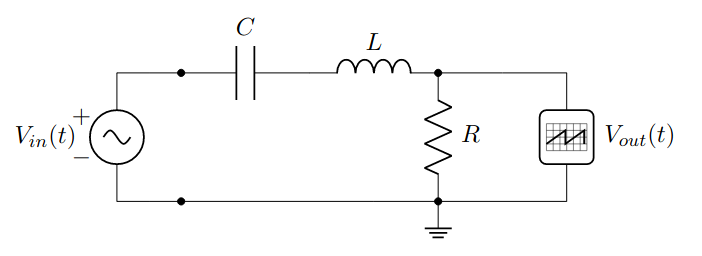
\includegraphics[width = 6 cm]{circuito.png}
            \caption{Circuito RC}
        \end{center}
    \end{figure}

    Nel primo esperimento è stato dato in ingresso a questa rete un segnale sinusoidale con offset nullo e 
    tensione picco-picco $V^{pp}_{in} = 5V$, di cui però è stata variata la frequenza più volte per ottenere diverse misurazioni
    di ampiezza e sfasamento della tensione d'uscita sul resistore, quindi $\mathbf{V_R}$.
    Una volta ottenute le misurazioni è possibile approssimare la funzione di trasferimento sperimentale $H_{sp}(j\omega)$
    e confrontarla con la funzione di trasferimento teorica $H(j\omega)$.\par
    È stata ripetuta questa procedura dopo aver sostituito il resistore corrente con uno avente una resistenza
    pari a $1k\Omega$. \par
    Durante il secondo esperimento è stato utilizzato lo stesso circuito, di cui sono state utilizzate 3 terne di valori di
    resistenze, induttanze e capacità. Dopo aver fornito in ingresso un'onda quadra di tensione picco-picco $V^{pp}_{in} = 2.5 V$
    e offset $V^{of}_{in} = 1.250 V$, è stato valutato l'andamento della tensione ai capi del resistore, al fine 
    di comprendere se il caso risultante fosse sovrasmorzato, sottosmorzato oppure criticamente smorzato. \par

    
    \section{Dati sperimentali}
    Primo esperimento : \par
    a: $R=10k\Omega$, $L=500mH$, $C=10nF$ \hspace{2.4cm} $b$: $R = 1k\Omega$,$L = 500mH $,$C = 10nF$
    
    \begin{table} [!ht]
        \begin{minipage}{.525\linewidth}
            %\caption{$a$: $R = 10k\Omega$,$L = 500mH $,$C = 10nF$}
            \centering
            \begin{tabular}{|c|c|c|}
                \hline
                \textit{Frequenza [Hz]} & \textit{Ampiezza [V]} & \textit{Sfasamento [ms]} \\
                \hline
                1 & $\longrightarrow 0$ & 196 \\
                \hline
                10 & 0.0324 & 27.8 \\
                \hline
                100 & 0.312 & 2.68 \\
                \hline
                1000 & 3 & 0.364 \\
                \hline
                2000 & 4.68 & 0.017 \\
                \hline
                2500 & 4.78 & 0.011 \\
                \hline
                3000 & 4.5 & 0.02 \\
                \hline
                5000 & 3.12 & 0.068 \\
                \hline
                10000 & 1.62 & 0.0192 \\
                \hline
                50000 & 0.093 & 0.0058 \\
                \hline
            \end{tabular}
        \end{minipage}
        \begin{minipage}{.525\linewidth}
            %\caption{$b$: $R = 10k\Omega$,$L = 500mH $,$C = 10nF$}
            \centering
            \begin{tabular}{|c|c|c|}
                \hline
                \textit{Frequenza [Hz]} & \textit{Ampiezza [V]} & \textit{Sfasamento [ms]} \\
                \hline
                1 & imp & imp \\
                \hline
                10 & 0.04 & 27.8 \\
                \hline
                100 & 0.031 & 2.68 \\
                \hline
                1000 & 0.38 & 0.364 \\
                \hline
                2000 & 2.24 & 0.017 \\
                \hline
                2500 & 2.3 & 0.011 \\
                \hline
                3000 & 1.108 & 0.02 \\
                \hline
                5000 & 0.396 & 0.068 \\
                \hline
                10000 & 0.163 & 0.0192 \\
                \hline
                50000 & 0.010 & 0.0058 \\
                \hline
            \end{tabular}
        \end{minipage}
    \end{table}

    Secondo esperimento (valori dei picchi visualizzati sull'oscilloscopio): \par
    \begin{tabular}{c l}
        $a$: & $R=10k\Omega$ \\
        & $L=500mH$ \\
        & $C=1nF$ \\
    \end{tabular}
    \hspace{2.5cm}
    \begin{tabular}{c l}
        $b$: & $R=10k\Omega$ \\
        & $L=500mH$ \\
        & $C=10nF$ \\
    \end{tabular}
    \hspace{2.25cm}
    \begin{tabular}{c l}
        $c$: & $R=10k\Omega$ \\
        & $L=100mH $ \\
        & $C=10nF$ \\
    \end{tabular}

    %px = [0.0032, 0.0081, 0.0151, 0.023, 0.0312]
    %$a$: $R = 10k\Omega$,$L = 500mH $,$C = 10nF$ \hspace{0.1cm} $c$: $R = 10k\Omega$,$L = 500mH $,$C = 10nF$ \hspace{0.1cm} $c$: $R = 10k\Omega$,$L = 500mH $,$C = 10nF$
    \begin{table} [!ht]
        \begin{minipage}{.34\linewidth}
            %\caption{$a$: $R = 10k\Omega$,$L = 500mH $,$C = 10nF$}
            \centering
            \begin{tabular}{|c|c|c|}
                \hline
                \textit{Tensione [V]} & \textit{Tempo [$\mu s$]} \\
                \hline
                0.8 & 32 \\
                \hline
                0.36 & 98 \\
                \hline
                0.2 & 172 \\
                \hline
                0.06 & 238 \\
                \hline
                0.06 & 312 \\
                \hline
            \end{tabular}
        \end{minipage}
        \begin{minipage}{.34\linewidth}
            %\caption{$b$: $R = 10k\Omega$,$L = 500mH $,$C = 10nF$}
            \centering
            \begin{tabular}{|c|c|}
                \hline
                \textit{Tensione [V]} & \textit{Tempo [$\mu s$]} \\
                \hline
                1.6 & 78 \\            
                \hline
            \end{tabular}
        \end{minipage}
        \begin{minipage}{.34\linewidth}
            %\caption{$c$: $R = 10k\Omega$,$L = 500mH $,$C = 10nF$}
            \centering
            \begin{tabular}{|c|c|}
                \hline
                \textit{Ampiezza [V]} & \textit{Tempo [$\mu s$]} \\
                \hline
                2.160 & 24 \\ 
                \hline
                1.88 & 48 \\
                \hline
                1.24 & 86 \\
                \hline
                0.8 & 132 \\         
                \hline
            \end{tabular}
        \end{minipage}
    \end{table}


    \section{Elaborazione dati}
    Primo esperimento:
    \begin{equation}
        \begin{split}
            H(j\omega) = \frac{\mathbf{V}_{out}}{\mathbf{V}_{in}}
            \hspace{0.5cm} dove \hspace{0.5cm} \mathbf{V}_{out} = \mathbf{I} \cdot \mathbf{Z_{R}} = \frac{\mathbf{V_{in}}}{\mathbf{Z_R} + \mathbf{Z_C} + \mathbf{Z_L}}
            \cdot \mathbf{Z_R}
            \\
            H(j\omega) =  \frac{1}{1+\frac{\mathbf{Z_C}}{\mathbf{Z_R}} + \frac{\mathbf{Z_R}}{\mathbf{Z_C}}}
            = \frac{1}{1+\frac{j}{R} \cdot \bigl (\omega L - \frac{1}{\omega C} \bigr )} = 
            \frac{1 - \frac{j}{R} \cdot \bigl (\omega L - \frac{1}{\omega C} \bigr )}{1 + \frac{1}{R^2} \cdot \bigl (\omega L - \frac{1}{\omega C} \bigr )}
            \\
            |H(j\omega)| = \sqrt{H(j\omega) \cdot \overline{H(j\omega)}} = \frac{1}{1 + \frac{1}{R^2} \cdot \bigl (\omega L - \frac{1}{\omega C} \bigr )} =
            \frac{1}{1+\frac{1}{R^2}\cdot\frac{L}{C}\cdot(\frac{\omega}{\omega_0} - \frac{\omega}{\omega})} 
            \\
            \phi_{H(j\omega)}(j\omega) = tan^{-1} \Bigl (\frac{Im(H(j\omega))}{Re(H(j\omega))}\Bigr )
            = tan^{-1} \Bigl (-\frac{1}{R} \cdot (\omega L - \frac{1}{\omega C})\Bigr )
        \end{split}
    \end{equation}

    \begin{center}
    Pongo $Q^2 = \frac{1}{R} \cdot \frac{L}{C}$ e $\omega_0 = \frac {1}{\sqrt{LC}}$
    \end{center}

    \begin{equation}
        \begin{split}
            |H(j\omega)| = \frac{1}{1 + Q^2 \cdot (\frac{\omega}{\omega_0} - \frac{\omega_0}{\omega})}
            \hspace{1cm}
            \phi_{H(j\omega)}(j\omega) = tan^{-1} \Bigl (-Q \cdot(\frac{\omega}{\omega_0} - \frac{\omega}{\omega_0}) \Bigr )
        \end{split}
    \end{equation}

    \begin{minipage}{.625\linewidth}
        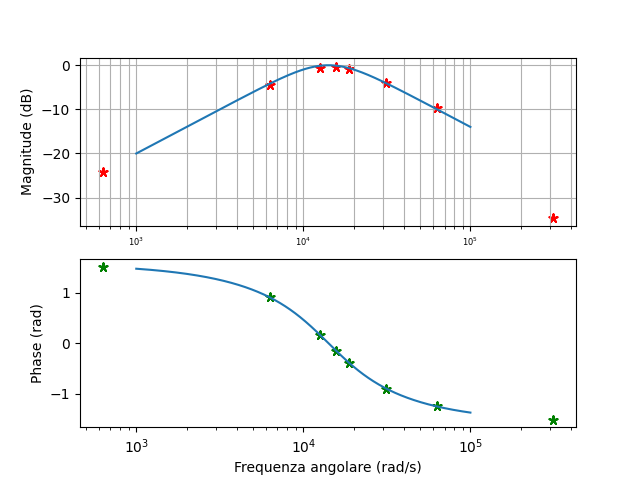
\includegraphics[width = 10.5 cm]{bode.png}
        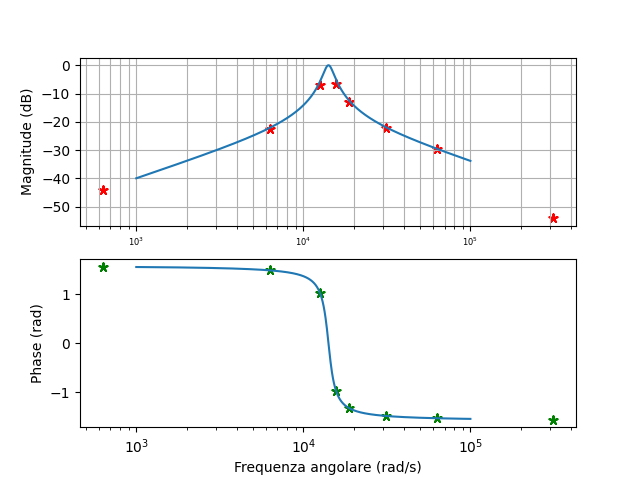
\includegraphics[width = 10.5 cm]{bode2.png}
    \end{minipage}
    \begin{minipage}{.4\linewidth}
        Primo caso:\par
        $Q^2=\frac{1}{10k\Omega} \cdot \frac{500mH}{10nF} = $ \par
        $\omega_0 = \frac{1}{\sqrt{500mH\cdot 10nF}}$ = 
        \\ \par
        Secondo caso:\par
        $Q^2=\frac{1}{1k\Omega} \cdot \frac{500mH}{10nF} = $ \par
        $\omega_0 = \frac{1}{\sqrt{500mH \cdot 10nF}}$ = 
    \end{minipage}

    \newpage
    Secondo esperimento: \par
    \begin{minipage}{.34\linewidth}
    \begin{math}
        KCL: I(t) = I_C(t) = I_L(t) = I_R(t) \\
        KVL: V_C(t) + V_L(t) + V_R(t) = V_S(t) \\
        \\
        V_C(t) + L\frac{dI_L(t)}{dt} + I_R(t)R = V_S(t) \hspace{1cm} I_C(t) = C\frac{dV_C(t)}{dt} \\
        \\
        V_C(t) + LC\frac{d^2V_C(t)}{dt^2} + RC\frac{dV_C(t)}{dt} = V_S(t) \\
        \\
        \ddot{V_C(t)} + \frac{R}{L}\dot{V_C(t)} +\frac{1}{LC}V_C(t) = \frac{V_S(t)}{LC} \\
        \\
        \ddot{V_C(t)} + 2\alpha \dot{V_C(t)} + {\omega_0}^2 V_C = 0 \\
        dove \hspace{0.5cm} \alpha = \frac{R}{2L} \hspace{0.5cm} \omega_0 = \frac{1}{\sqrt{LC}} \\
        \\
        \textit{Caso 1:} \hspace{0.5cm} R = 10K\Omega \hspace{0.5cm} L = 500mH \hspace{0.5cm} C = 1nF \\
        \alpha < \omega_0 \hspace{0.5cm} \textit{Caso sottosmorzato} \\
        \\
        \textit{Caso 2:} \hspace{0.5cm} R = 10K\Omega \hspace{0.5cm} L = 500mH \hspace{0.5cm} C = 10nF \\
        \alpha < \omega_0 \hspace{0.5cm} \textit{Caso sottosmorzato} \\
        \\
        \textit{Caso 3:} \hspace{0.5cm} R = 10K\Omega \hspace{0.5cm} L = 100mH \hspace{0.5cm} C = 10nF \\
        \alpha > \omega_0 \hspace{0.5cm} \textit{Caso sovrasmorzato} \\
        \\
    \end{math}
    \end{minipage}
    \hspace{0.5 cm}
    \begin{minipage}{.4\linewidth}
        \hspace{0.5 cm}
        Primo caso : \par
        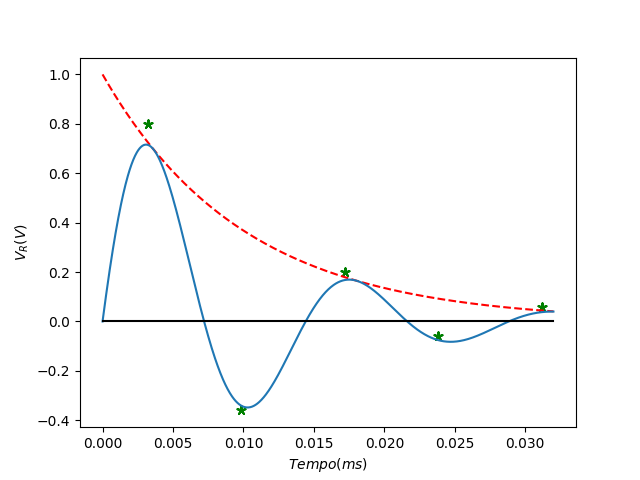
\includegraphics[width = 9 cm]{secondoese.png}
        \par
        \hspace{0.5 cm} Dove \color{blue} $V_R(t) = Ae^{-\alpha t} cos(\omega_d t + \phi)$
    \end{minipage}

    \section{Conclusione}
    Possiamo notare nel primo esperimento che i punti si sovrappongono quasi perfettamente al diagramma di Bode teorico.\par
    Mentre nel secondo esperimento (trovare la frequenza di oscillazione)
\end{document}